\section{Konzept Propeller}

\begin{figure}[h!]
	\centering
	\begin{subfigure}[b]{0.45\textwidth}
		\includegraphics[width=\textwidth]{../../fig/Drehrad_Mitnehmer.jpg}
		\caption{Drehrad mit Mitnehmer}
	\end{subfigure}
	\begin{subfigure}[b]{0.45\textwidth}
		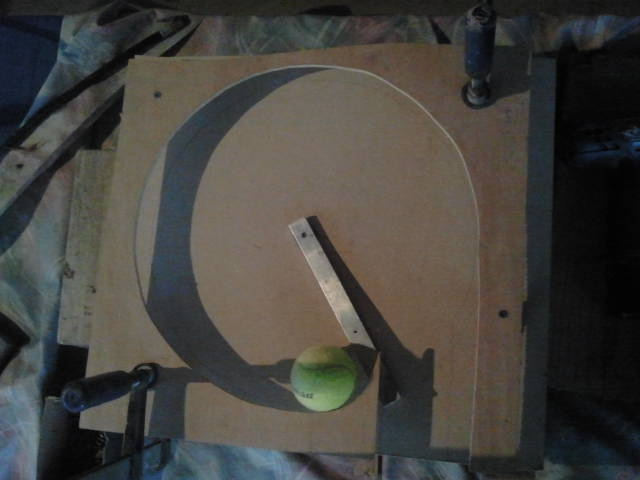
\includegraphics[width=\textwidth]{../../fig/prototyp_propeller.jpg}
		\caption{Prototyp Drehrad mit Mitnehmer}
	\end{subfigure}
	\caption{Testaufbau}
	\label{fig:drehrad_mitnehmer}
\end{figure}

\subsection{Idee}
Bei dieser Variante werden die Tennisbälle mit einem Mitnehmer innerhalb von einer Umdrehung auf die nötige Abwurfgeschwindigkeit gebracht. Die Bälle werden nacheinander dem Mitnehmer zugeführt. Es besteht die Möglichkeit, dass der Teller mit dem Mitnehmer horizontal oder vertikal im Gerät eingebaut wird. Da eine hohe Umfangsgeschwindigkeit nötig ist, um den Ball auf die geforderte Geschwindigkeit zu Beschleunigen müssen die Bälle in kurzer Zeit dem Mitnehmer zugeführt werden. Die Bälle werden in Umfangsrichtung mit einer Führung bis zur Abschussposition in Position gehalten. Als Antrieb wird ein Getriebemotor eingesetzt.  

\subsection{Annahmen}
Ob das Konzept mit dem Mitnehmer funktioniert, wurde mit einem Prototyp überprüft. Dabei wurde ein Motor verwendet, welcher die geforderte Drehzahl nicht erreicht. Dementsprechend war die erreichte Wurfdistanz nur rund 40 cm. Dies sollte mit einem passenden Motor kein Problem mehr darstellen. Beim Versuchsaufbau wurde der Tennisball nur in Umfangsrichtung und auf einer Platte geführt. Dies führte dazu, dass der Ball teilweise gegen oben aus der Vorrichtung heraussprang. Dieses Problem kann mit einer geschlossenen Bauweise behoben werden.   

\subsection{Vor- und Nachteile}

Vorteile: Diese Art von Abwurfvorrichtung ist weitgehend unabhängig von der Ballgrösse (im vorgegebenen Bereich gemäss Aufgabenstellung). Die Bälle können in einem sehr geringen Zeitrahmen beschleunigt werden. Dadurch ist diese Variante sehr schnell, was die Abwurfgeschwindigkeit betrifft.   

Nachteile: Beim Versuchsaufbau landeten die Tennisbälle in einem Feld von 30x30 cm. Somit liegt die Genauigkeit unter unseren Ansprüchen. Die benötigte Umfangsgeschwindigkeit ist so hoch, dass die Bälle nicht nur mittels der Gewichtskraft zugeführt werden können. Dies erfordert eine aufwendige Magazinkonstruktion. Damit für alle Tennisbälle identische Abwurfbedingungen vorhanden sind, muss der Motor zuerst auf die gewünschte Drehzahl gebracht werden. Dies führt wiederum zu einer aufwendigen Magazinkonstruktion. Durch die Konstruktion mit den Führungen wird das Gewicht der Konstruktion eher hoch.  
